\chapter{玻尔兹曼权重、配分函数与理想气体}

\lectureoverview{我们通过在固定归一化和固定平均能量的条件下最大化熵，推导出平衡概率分布。随后，配分函数通过微分给出平均能量、熵和温度。理想气体提供了第一个完整例子，接着是引力推广以及能量涨落的预告。}

\section{约束熵问题}

从大量\(\mathcal N\)个相同、相互作用极弱的同一子系统的复本开始。若\(n_i\)个复本占据第\(i\)个态，则
\begin{equation}
 p_i=\frac{n_i}{\mathcal N},
 \qquad
 \sum_i p_i=1.
 \label{eq:sm4-occupation-probability}
\end{equation}
上一讲的多项式计数给出每个复本的熵，
\begin{equation}
 S[p]=-\sum_i p_i\log p_i.
 \label{eq:sm4-entropy}
\end{equation}
值得将其视为所有变量\(p_1,p_2,\ldots\)的普通函数。正是其简单的可加形式使计算成为可能。

复本集合具有固定的总能量\(\mathcal N E\)，其中\(E\)是每个复本的平均能量。因此第二个约束为
\begin{equation}
 \sum_i p_iE_i=E.
 \label{eq:sm4-energy-constraint}
\end{equation}
能级\(E_i\)属于该子系统；右侧的数\(E\)是它们的概率加权平均值。在\eqref{eq:sm4-occupation-probability}和\eqref{eq:sm4-energy-constraint}的约束下最大化\eqref{eq:sm4-entropy}，选出压倒性最可能的占据分数。

为方便起见，最小化\(-S=\sum_i p_i\log p_i\)。为每个约束引入一个拉格朗日乘子：
\begin{equation}
 \begin{aligned}
 \Phi[p;\alpha,\beta]
 &=\sum_i p_i\log p_i\\
 &\quad+\alpha\left(\sum_i p_i-1\right)\\
 &\quad+\beta\left(\sum_i p_iE_i-E\right).
 \end{aligned}
 \label{eq:sm4-augmented-functional}
\end{equation}
名称\(\alpha\)和\(\beta\)尚不是物理假设。在此阶段，它们只是为强制施加两个约束所需的两个数。

\begin{classroomqa}
\audiencequestion{增广函数也是\(\alpha\)和\(\beta\)的函数吗？}
\lecturerresponse{是的。对\(\alpha\)和\(\beta\)变分可恢复这两个约束。然而，对于当前的计算，我们保持这些乘子固定，并对概率\(p_i\)变分。它们的值随后由归一化和给定的平均能量确定。
\lecturetimestamp{00:09:32--00:09:49}}
\end{classroomqa}

\begin{figure}[t]
\centering
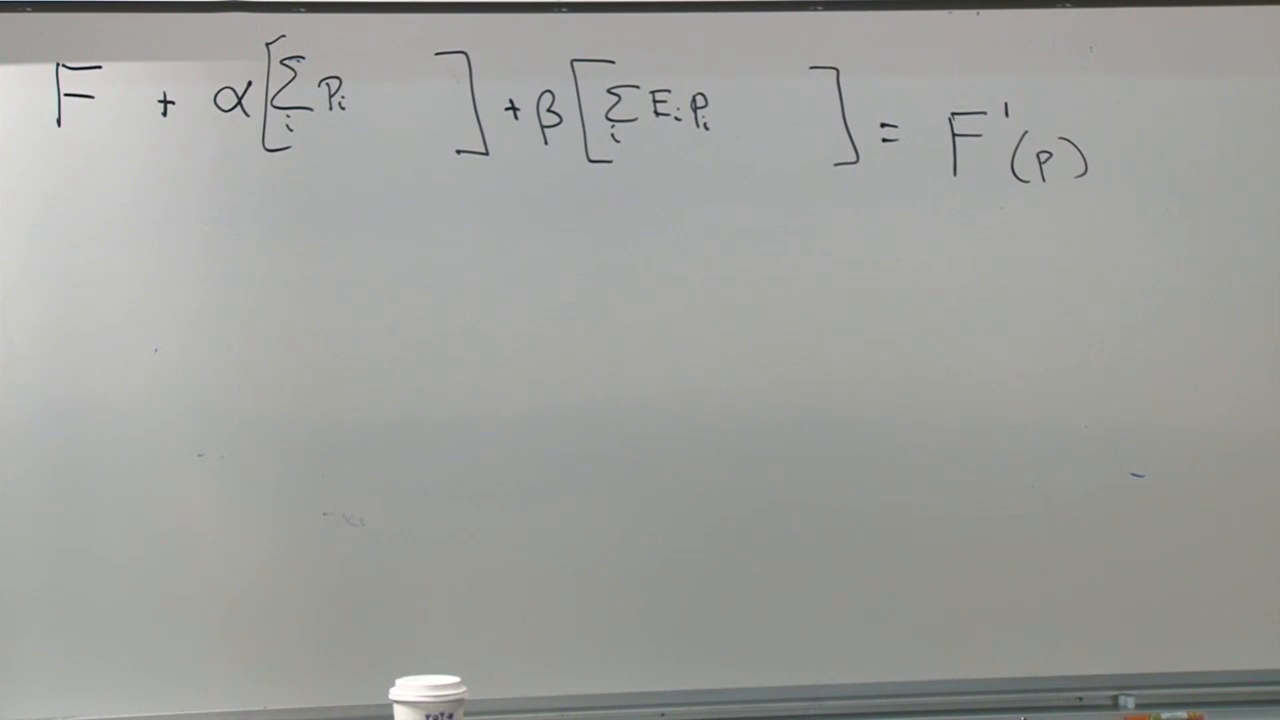
\includegraphics[width=0.92\textwidth]{lecture_04_figure_02.png}
\caption{在概率变分下为常数的项被略去后的增广熵泛函。}
\lectureframe{00:10:56}
\end{figure}

对某个概率求导时，项\(-\alpha\)和\(-\beta E\)不贡献任何东西。这就是黑板上可见的简写泛函。它们仍然是\eqref{eq:sm4-augmented-functional}的一部分；只是对这个特定的导数而言变得无关紧要。

\section{玻尔兹曼分布}

任选一个概率。本讲选择\(p_7\)，部分是因为\(1\)看起来太特殊，而\(7\)是个幸运数字。这个选择无关紧要。所需的微积分仅为
\begin{equation}
 \frac{d}{dp_i}\bigl(p_i\log p_i\bigr)=\log p_i+1.
\end{equation}
因此
\begin{equation}
 \frac{\partial\Phi}{\partial p_i}
 =\log p_i+1+\alpha+\beta E_i=0.
 \label{eq:sm4-stationarity}
\end{equation}
解出\(p_i\)，
\begin{align}
 \log p_i&=-(1+\alpha)-\beta E_i,\\
 p_i&=e^{-(1+\alpha)}e^{-\beta E_i}.
\end{align}
第一个因子与态标号无关。将其写为\(1/Z\)：
\begin{equation}
 p_i=\frac{e^{-\beta E_i}}{Z}.
 \label{eq:sm4-boltzmann-weight}
\end{equation}

这是第一个突如其来的收获。一个常规的约束导数产生了指数定律。相对概率满足
\begin{equation}
 \frac{p_i}{p_j}=e^{-\beta(E_i-E_j)}.
 \label{eq:sm4-relative-weight}
\end{equation}
乘子\(\beta\)控制概率随能量下降的快慢。大的正\(\beta\)使分布集中在最低能级附近；小的正\(\beta\)将可观的权重散布到能谱中更高的位置。我们已经可以看出，改变\(\beta\)会改变平均能量，尽管它与逆温度的等同仍有待证明。

\section{归一化与配分函数}

归一化确定了与态无关的因子：
\begin{equation}
 1=\sum_i p_i
 =\frac{1}{Z}\sum_i e^{-\beta E_i},
\end{equation}
所以
\begin{equation}
 Z(\beta)=\sum_i e^{-\beta E_i}.
 \label{eq:sm4-partition-function}
\end{equation}
这就是正则配分函数。它最初作为归一化常数出现，但这一描述严重低估了它的作用。一旦\(Z(\beta)\)已知，热力学量便可由其导数得到。

\eqref{eq:sm4-partition-function}中的能级是输入量。它们来自系统的力学以及固定的外部条件：盒子的体积和形状、磁场或电场，以及任何其他控制参数。改变控制参数会改变能谱，从而改变\(Z\)。对于当前的计算，这些参数以及集合\(\{E_i\}\)都保持固定。

\begin{classroomqa}
\audiencequestion{指数草图的坐标轴究竟代表什么？纵坐标是某个特定的\(p_i\)吗？}
\lecturerresponse{所绘制的高度是赋予某个能级的概率，而水平方向的排序既可以读作态标号\(i\)，也可以更物理地读作能量\(E_i\)。每个态都有固定的能量。大的\(\beta\)使概率随该能量急剧下降；在\(\beta=0\)附近，权重在可及能级上几乎平坦。
\lecturetimestamp{00:19:39--00:20:09}}
\end{classroomqa}

\section{隐藏在配分函数中的平均能量}

第二个约束条件确定\(\beta\)：
\begin{equation}
 E=\sum_i p_iE_i
 =\frac{1}{Z}\sum_i E_i e^{-\beta E_i}.
 \label{eq:sm4-mean-energy}
\end{equation}
与其重新计算这个加权求和，不如对
\eqref{eq:sm4-partition-function}求导：
\begin{equation}
 \frac{dZ}{d\beta}
 =-\sum_i E_i e^{-\beta E_i}.
\end{equation}
与\eqref{eq:sm4-mean-energy}比较可得
\begin{equation}
 E(\beta)
 =-\frac{1}{Z}\frac{dZ}{d\beta}
 =-\frac{d\log Z}{d\beta}.
 \label{eq:sm4-energy-logz}
\end{equation}
取自然对数，因为它的导数正好给出因子
\(1/Z\)。

\begin{figure}[t]
\centering
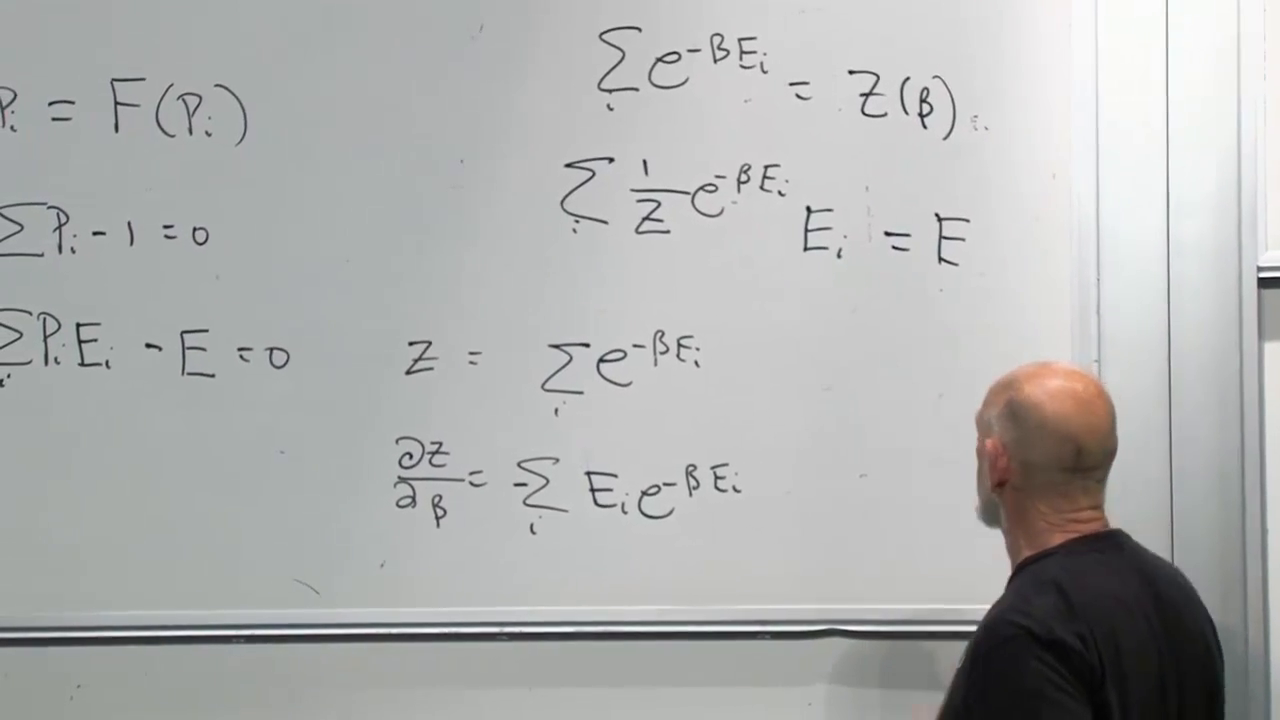
\includegraphics[width=0.82\textwidth]{lecture_04_figure_03.png}
\caption{归一化条件、平均能量约束以及配分函数的导数一同出现在黑板上。}
\lectureframe{00:26:24}
\end{figure}

\begin{classroomqa}
\audiencequestion{黑板下方的方程是关于\(Z\)的新方程，还是由它上方的定义得到的？}
\lecturerresponse{它是对定义
\(Z=\sum_i e^{-\beta E_i}\)求导得到的。求导会带下
\(-E_i\)。再将结果除以\(Z\)，就重现了定义平均能量的那个加权求和。
\lecturetimestamp{00:25:58--00:26:37}}
\end{classroomqa}

\begin{classroomqa}
\audiencequestion{
\(dZ/d\beta=-E Z\)是否使\(Z\)成为微分算子的本征函数？}
\lecturerresponse{并非通常意义上的本征函数。本征值方程应当是一个常数乘以\(Z\)，而这里
\(E=E(\beta)\)。这个方程告诉我们平均能量作为
\(\beta\)的函数；它不是一个固定本征值问题。
\lecturetimestamp{00:28:49--00:29:43}}
\end{classroomqa}

\eqref{eq:sm4-energy-logz}的简洁性具有欺骗性。能谱可能很复杂，计算\(Z\)也可能很困难，但一旦求出这个单一函数，平均能量只需一次求导即可得到。这种模式在统计力学中反复出现：以正确的顺序施加基本运算，就能得到直接猜测会很困难的结果。

\begin{classroomqa}
\audiencequestion{\(E\)是所有复本的总能量，还是每个盒子的平均能量？}
\lecturerresponse{它是一个盒子的平均能量。复本集合的总能量为\(\mathcal N E\)。之后，当系统本身被选为一个包含\(N\)个气体粒子的完整盒子时，\(E\)将表示整个气体样本的能量。
\lecturetimestamp{00:30:55--00:31:10}}
\end{classroomqa}

\begin{classroomqa}
\audiencequestion{我们可以对
\(\sum_i e^{-\beta E_i}\)逐项取对数吗？}
\lecturerresponse{不可以。对数把乘积变成求和，而不是把求和变成对数之和：
\[
 \log\!\left(\sum_i e^{-\beta E_i}\right)
 \ne \sum_i\log\!\left(e^{-\beta E_i}\right).
\]
这一区别在之后会变得有用，那时独立子系统的配分函数会相乘。
\lecturetimestamp{00:31:10--00:31:58}}
\end{classroomqa}

\section{什么固定，什么允许变化？}

同一组公式中存在若干层次的变量，课堂讨论有意将它们区分开来。

\begin{itemize}
 \item 概率\(p_i\)是原始的未知量。
 \item 一旦系统及其控制参数给定，能级\(E_i\)就是固定的。
 \item 乘子\(\alpha\)已被吸收到归一化
 \(Z=e^{1+\alpha}\)中。
 \item 对于给定的平均能量\(E\)，约束条件确定一个数
 \(\beta\)。然而，在一族平衡态中，既可以使用
 \(E=E(\beta)\)，也可以使用\(\beta=\beta(E)\)。
\end{itemize}

\begin{classroomqa}
\audiencequestion{如果乘子是数，为什么\(\beta\)和
\(E\)现在被当作变量处理？}
\lecturerresponse{对于单个约束问题，它们确实是数。但我们可以比较许多具有相同能谱和不同给定平均能量的平衡问题。在这一族中，\(\beta\)随
\(E\)变化。固定\(E\)就确定\(\beta\)；固定\(\beta\)就确定
\(E\)。这是同一关系的两种读法。
\lecturetimestamp{00:31:58--00:33:27}}
\end{classroomqa}

\begin{classroomqa}
\audiencequestion{\(\alpha\)消失了吗？}
\lecturerresponse{消失的只是它的名字。定义
\(e^{-(1+\alpha)}=1/Z\)把它吸收到\(Z\)中。同时保留\(\alpha\)
和\(Z\)会把同一个归一化参数计算两次。
\lecturetimestamp{00:33:29--00:33:49}}
\end{classroomqa}

能量不必是唯一的守恒量。如果总动量、粒子数、角动量或其他量受到约束，它的期望值就会获得自己的乘子。这种扩展改变了系综，但不改变方法。

\begin{classroomqa}
\audiencequestion{只固定平均能量是否对系统作了过多假设？}
\lecturerresponse{它假设在当前问题中不需要以其他守恒量为条件。例如，如果总动量也被固定，那就再加一个约束和另一个拉格朗日乘子。相比之下，体积、形状和外场在这里是控制参数：它们被固定，并决定能级本身。
\lecturetimestamp{00:33:51--00:35:50}}
\end{classroomqa}

\begin{classroomqa}
\audiencequestion{\(\alpha\)是否应作为能量的另一个自变量出现，而\(Z\)是否依赖于能级\(E_i\)？}
\lecturerresponse{\(\alpha\)已经包含在\(Z\)中，因此它不是独立的自变量。配分函数当然既依赖于固定的谱，也依赖于\(\beta\)。改变控制参数会改变\(E_i\)，从而改变\(Z\)；在当前的\(\beta\)导数运算中，谱保持固定。
\lecturetimestamp{00:35:52--00:37:10}}
\end{classroomqa}

\begin{classroomqa}
\audiencequestion{我们是在改变各个能级\(E_i\)，还是在改变平均能量\(E\)？}
\lecturerresponse{各个能级保持固定。平均能量发生变化，是因为概率发生了变化。因此，这一族由\(E\)参数化，或等价地由\(\beta\)参数化，而始终使用同一组能级\(\{E_i\}\)。
\lecturetimestamp{00:37:12--00:39:04}}
\end{classroomqa}

实际上，温度往往比气体的总能量容易测量得多。我们可以插入温度计；称量相对论质量差并援引\(E=mc^2\)虽然正确，却毫无帮助。为了使\(\beta\)具有可操作性，我们现在必须把它与温度的热力学定义联系起来。

\section{温度之前的熵}

从逻辑上说，熵在先。将玻尔兹曼概率代入\eqref{eq:sm4-entropy}：
\begin{equation}
 \log p_i=-\beta E_i-\log Z.
\end{equation}
于是
\begin{align}
 S
 &=-\sum_i p_i\log p_i\\
 &=\beta\sum_i p_iE_i+\log Z\sum_i p_i\\
 &=\beta E+\log Z.
 \label{eq:sm4-entropy-logz}
\end{align}
归一化求和提供了最后的因子一。这也是亥姆霍兹自由能的最初迹象，因为之后在\(k_B=1\)的单位制下，\(F_{\mathrm H}=-T\log Z\)。

\begin{classroomqa}
\audiencequestion{第一项中的因子\(1/Z\)到哪里去了？}
\lecturerresponse{它已经是\(p_i\)的一部分。求和\(\sum_i p_iE_i\)包含完整的归一化概率，并且按定义就是平均能量\(E\)。
\lecturetimestamp{00:43:19--00:43:26}}
\end{classroomqa}

\begin{classroomqa}
\audiencequestion{\(S=\beta E+\log Z\)中是否应该有一个负号？}
\lecturerresponse{不。熵以一个负号开头，而\(\log p_i=-\beta E_i-\log Z\)还包含另外两个负号。它们产生\eqref{eq:sm4-entropy-logz}中显示的两个正项。
\lecturetimestamp{00:45:53--00:46:03}}
\end{classroomqa}

温度在热力学上由
\begin{equation}
 dE=T\,dS,
 \qquad
 \frac{1}{T}=\frac{dS}{dE},
 \label{eq:sm4-temperature-definition}
\end{equation}
定义，其中所有其他控制参数保持固定。直接对\eqref{eq:sm4-entropy-logz}关于\(E\)求导的第一次尝试很快就会变得杂乱，因为\(\beta\)也依赖于\(E\)。取全微分更简洁：
\begin{align}
 dS
 &=\beta\,dE+E\,d\beta
   +\frac{d\log Z}{d\beta}\,d\beta\\
 &=\beta\,dE+E\,d\beta-E\,d\beta\\
 &=\beta\,dE.
 \label{eq:sm4-entropy-differential}
\end{align}
消去利用了\eqref{eq:sm4-energy-logz}。将\eqref{eq:sm4-entropy-differential}与\eqref{eq:sm4-temperature-definition}比较，得到
\begin{equation}
 T=\frac{1}{\beta},
 \qquad
 \beta=\frac{1}{T}.
 \label{eq:sm4-beta-temperature}
\end{equation}

\begin{figure}[t]
\centering
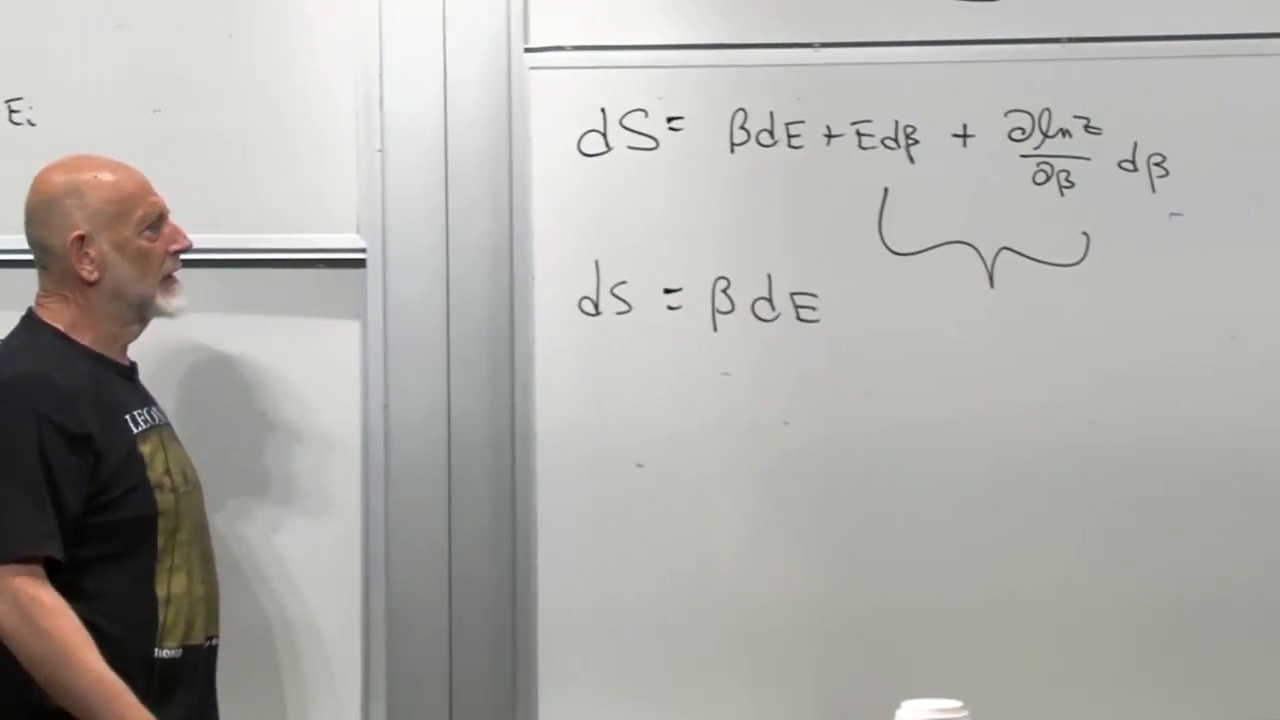
\includegraphics[width=0.82\textwidth]{lecture_04_figure_04.png}
\caption{两个\(d\beta\)项相消，剩下\(dS=\beta\,dE\)。}
\lectureframe{00:50:48}
\end{figure}

\begin{classroomqa}
\audiencequestion{这种相消是否错误地假设了\(\log Z\)与能量或温度无关？}
\lecturerresponse{不。对于固定的谱，只有一个独立的热力学参数。我们可以写出\(Z=Z(\beta)\)，然后沿平衡族将\(\beta=\beta(E)\)视为函数。全微分保留了完整的\(d\beta\)依赖关系，而恒等式\(d\log Z/d\beta=-E\)正是使相消成立的原因。
\lecturetimestamp{00:52:04--00:52:44}}
\end{classroomqa}

在大部分计算中，温度以能量单位计量，因此\(k_B=1\)。恢复实验室单位后，
\begin{equation}
 \beta=\frac{1}{k_B T_{\mathrm K}},
 \label{eq:sm4-beta-laboratory}
\end{equation}
其中\(T_{\mathrm K}\)是以开尔文表示的绝对温度。通常方便地写出\(T_{\mathrm e}=k_BT_{\mathrm K}\)，然后使用\(\beta=1/T_{\mathrm e}\)。

\begin{classroomqa}
\audiencequestion{对于一定体积的气体，系统是一个分子还是整个集合？}
\lecturerresponse{这取决于系统如何定义。这里系统将是整箱气体，因此\(E\)是其所有分子的能量。对于足够稀薄的理想气体，一个分子也可以被视为一个子系统，因为粒子之间不发生相互作用；下面的因子化将展示这两种描述之间的关系。
\lecturetimestamp{00:53:32--00:54:49}}
\end{classroomqa}

现在可以汇总正则系综的各个恒等式：
\begin{align}
 p_i&=\frac{e^{-\beta E_i}}{Z},&
 Z(\beta)&=\sum_i e^{-\beta E_i},\label{eq:sm4-canonical-pair}\\
 E&=-\frac{d\log Z}{d\beta},&
 S&=\beta E+\log Z,&
 T&=\frac{1}{\beta}.
 \label{eq:sm4-canonical-identities}
\end{align}

\section{经典理想气体}

取\(N\)个质量为\(m\)的全同点粒子，置于体积为\(V\)的盒子中。当粒子之间的相互作用可以忽略时，气体是理想的。这可能是一个好的近似，因为力很弱，或者因为气体足够稀薄，近距离相遇很少发生。

一个经典微观态由所有位置和动量指定：
\begin{equation}
 (\bm q_1,\ldots,\bm q_N;\bm p_1,\ldots,\bm p_N).
\end{equation}
有\(3N\)个位置坐标和\(3N\)个动量坐标，因此该状态是\(6N\)维相空间中的一个点。在没有相互作用的情况下，哈密顿量为
\begin{equation}
 H(\bm p)=\sum_{a=1}^{N}\frac{\bm p_a^2}{2m}
 =\sum_{\mu=1}^{3N}\frac{p_\mu^2}{2m}.
 \label{eq:sm4-ideal-hamiltonian}
\end{equation}

\begin{classroomqa}
\audiencequestion{有\(3N\)个粒子吗？对所有动量分量求和是否会重复计算状态？}
\lecturerresponse{有\(N\)个粒子和\(3N\)个动量分量。\eqref{eq:sm4-ideal-hamiltonian}中的求和对每个分量包含一个二次项。相空间积分随后对每个独立分量恰好积分一次，因此该乘积不会导致重复计数。
\lecturetimestamp{01:02:29--01:04:04}}
\end{classroomqa}

对于连续经典相空间，态求和变为
\begin{equation}
 Z_N
 =\frac{1}{N!\,h^{3N}}
 \int_{V^N}d^{3N}q
 \int_{\mathbb R^{3N}}d^{3N}p\,
 e^{-\beta H(\bm p)}.
 \label{eq:sm4-classical-partition}
\end{equation}
讲座聚焦于积分，并写出不带相空间单元\(h^{3N}\)的同一表达式。将其恢复使\(Z_N\)无量纲，并记录了经典态计数的量子起源。由于\(h\)与\(\beta\)无关，它不改变下文所用的能量导数。

位置积分是直接的。哈密顿量与位置无关，每个粒子可以位于盒子中的任何位置：
\begin{equation}
 \int_{V^N}d^{3N}q=V^N.
\end{equation}
动量积分分解为\(3N\)个相同的一维高斯积分：
\begin{equation}
 Z_N
 =\frac{V^N}{N!\,h^{3N}}
 \left[
  \int_{-\infty}^{\infty}dp\,
  e^{-\beta p^2/(2m)}
 \right]^{3N}.
 \label{eq:sm4-factorized-gas}
\end{equation}

因子\(1/N!\)标识了仅因相同粒子的置换而不同的构型。对于固定\(N\)和\(V\)下的平均能量，它只对\(\log Z_N\)贡献一个与\(\beta\)无关的常数，因此在\(-\partial/\partial\beta\)下消失。但它并非在每个问题中都可随意丢弃：与\(h^{3N}\)一起，它对于无量纲配分函数、广延熵和一致化学势是必不可少的。

现在令
\begin{equation}
 x=\sqrt{\frac{\beta}{2m}}\,p,
 \qquad
 dp=\sqrt{\frac{2m}{\beta}}\,dx.
\end{equation}
高斯积分变为
\begin{align}
 \int_{-\infty}^{\infty}dp\,e^{-\beta p^2/(2m)}
 &=
 \sqrt{\frac{2m}{\beta}}
 \int_{-\infty}^{\infty}dx\,e^{-x^2}\\
 &=\sqrt{\frac{2\pi m}{\beta}}.
 \label{eq:sm4-gaussian}
\end{align}

\begin{figure}[t]
\centering
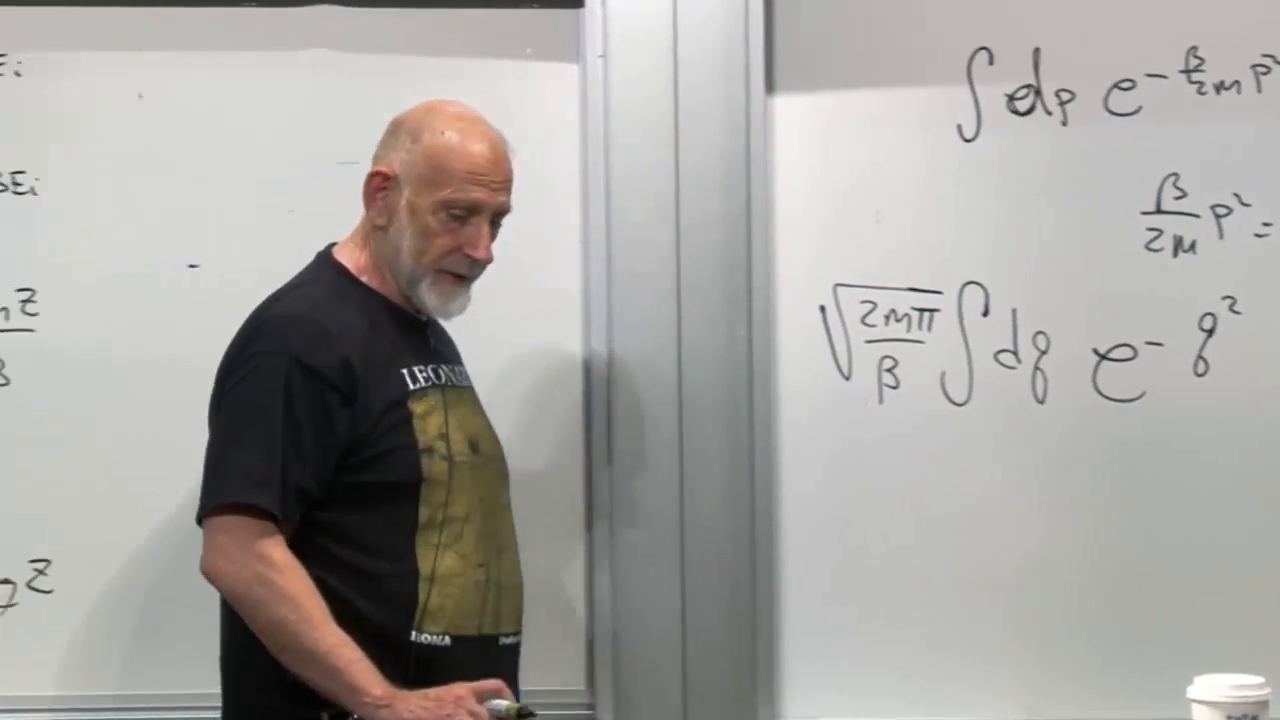
\includegraphics[width=0.82\textwidth]{lecture_04_figure_05.png}
\caption{通过一次重标度，动量积分被化为标准高斯积分。}
\lectureframe{01:13:12}
\end{figure}

代入\eqref{eq:sm4-factorized-gas}得到
\begin{equation}
 Z_N
 =\frac{V^N}{N!\,h^{3N}}
 \left(\frac{2\pi m}{\beta}\right)^{3N/2}.
 \label{eq:sm4-ideal-partition}
\end{equation}

\begin{figure}[t]
\centering
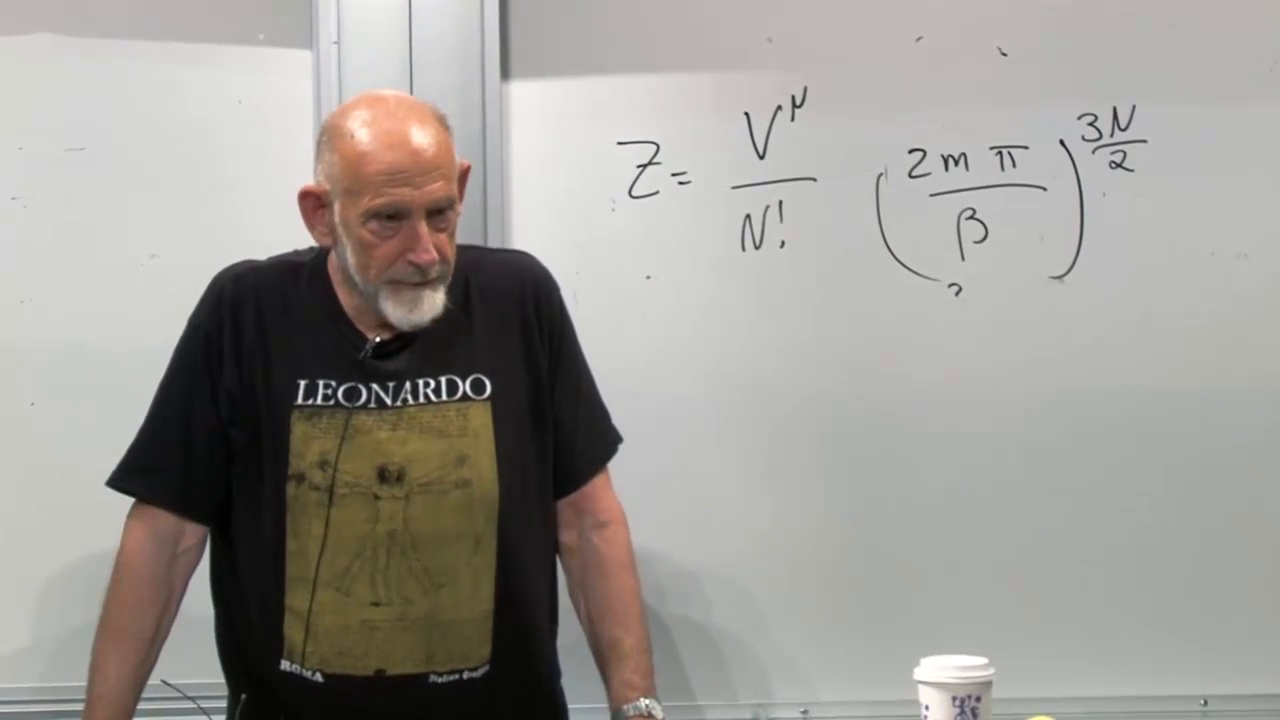
\includegraphics[width=0.78\textwidth]{lecture_04_figure_06.png}
\caption{黑板上完成的理想气体配分函数。相空间单元\(h^{3N}\)在\eqref{eq:sm4-ideal-partition}中被恢复。}
\lectureframe{01:14:38}
\end{figure}

用热德布罗意波长将同一结果打包是有用的
\begin{equation}
 \lambda_T=\frac{h}{\sqrt{2\pi mT}}
 \qquad (k_B=1).
\end{equation}
于是
\begin{equation}
 Z_N=\frac{1}{N!}\left(\frac{V}{\lambda_T^3}\right)^N.
 \label{eq:sm4-thermal-wavelength-form}
\end{equation}

对于宏观的\(N\)，斯特林公式给出
\begin{equation}
 N!\simeq N^Ne^{-N}\sqrt{2\pi N}.
\end{equation}
只保留主导指数依赖并定义\(\rho=N/V\)，
\begin{equation}
 \frac{V^N}{N!}
 \simeq
 \frac{1}{\sqrt{2\pi N}}
 \left(\frac{e}{\rho}\right)^N.
 \label{eq:sm4-density-rewrite}
\end{equation}
这是讲座中简洁的密度重写。平方根因子在\(\log Z_N\)中是次主导的，但这里将其显示出来，而不是悄悄丢弃。

\begin{classroomqa}
\audiencequestion{如果\(1/N!\)与\(\beta\)无关，它是否完全不起作用？}
\lecturerresponse{对于当前固定\(N\)和\(V\)下的平均能量导数，它不起作用，因为它对\(\log Z_N\)添加了一个与\(\beta\)无关的常数。它对于绝对熵和粒子数变化确实有影响。有限的导数陈述与更广泛的态计数陈述不应混淆。
\lecturetimestamp{01:27:01--01:27:51}}
\end{classroomqa}

\section{能量与均分}

乘积难以求导；对数将它们变为求和。由\eqref{eq:sm4-ideal-partition}，
\begin{equation}
 \log Z_N
 =-\frac{3N}{2}\log\beta+\text{\(\beta\)-independent terms}.
 \label{eq:sm4-log-ideal-partition}
\end{equation}
因此
\begin{equation}
 E
 =-\frac{\partial\log Z_N}{\partial\beta}
 =\frac{3N}{2\beta}
 =\frac{3N}{2}T.
 \label{eq:sm4-ideal-energy}
\end{equation}
每个粒子的能量为
\begin{equation}
 \frac{E}{N}=\frac{3}{2}T
 \qquad (k_B=1),
\end{equation}
或者，用实验室单位表示，
\begin{equation}
 \frac{E}{N}=\frac{3}{2}k_BT_{\mathrm K}.
 \label{eq:sm4-ideal-energy-lab}
\end{equation}

\begin{figure}[t]
\centering
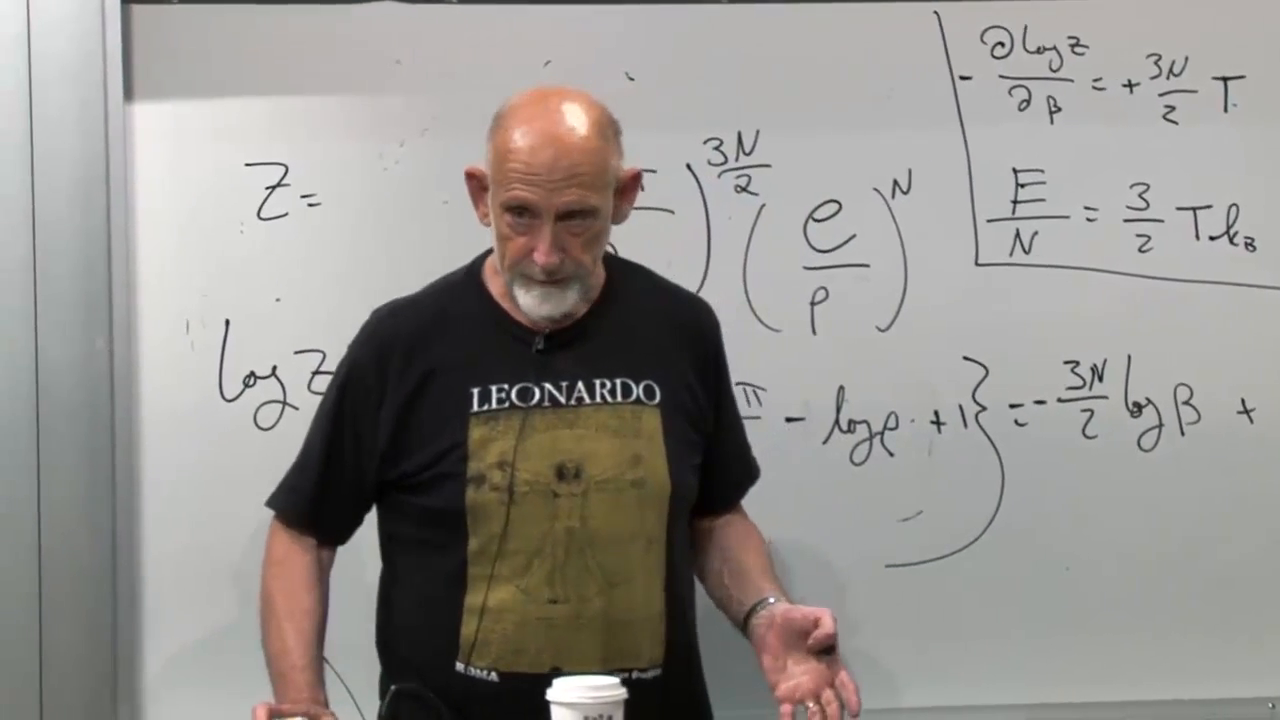
\includegraphics[width=0.84\textwidth]{lecture_04_figure_07.png}
\caption{只有\(-3N\log\beta/2\)项对理想气体能量有贡献，给出\(E/N=3T/2\)。}
\lectureframe{01:25:28}
\end{figure}

\begin{classroomqa}
\audiencequestion{玻尔兹曼常数如何进入能量公式？}
\lecturerresponse{理论家的温度\(T\)是一种能量。要使用开尔文，将其替换为\(k_BT_{\mathrm K}\)，得到\(E/N=3k_BT_{\mathrm K}/2\)。\(k_B\)的小数值将看似宏观的数值温度转换为单个分子的微观能量尺度。
\lecturetimestamp{01:24:58--01:26:01}}
\end{classroomqa}

3来自空间的三个方向。1/2来自每个高斯积分对\(1/\beta\)的平方根依赖。每个独立的二次动量坐标对平均能量贡献
\begin{equation}
 \frac{1}{2}T
\end{equation}
在\(d\)个空间维度中，同样的论证给出\(E/N=dT/2\)。这是均分定理的首次出现。

讲座末尾布置的熵计算由\(S=\beta E+\log Z_N\)得出。使用斯特林近似，
\begin{equation}
 \frac{S}{N}
 \simeq
 \log\!\left[
  \frac{V}{N}
  \left(\frac{2\pi mT}{h^2}\right)^{3/2}
 \right]
 +\frac{5}{2},
 \label{eq:sm4-sackur-tetrode}
\end{equation}
直到次主导的有限\(N\)修正。恢复\(k_B\)将右侧乘以\(k_B\)，并将\(T\)替换为\(k_BT_{\mathrm K}\)。结果清楚地表明，为什么从能量中消失的归一化因子对于熵是不可或缺的。

\section{将气体置于引力场中}

关于把盒子放在中子星上的问题引出了引力推广。在直面中子星之前，先考虑普通房间中的均匀场 \(g\)。取 \(y=0\) 位于底面积为 \(A\)、高度为 \(L\) 的盒子底部。哈密顿量变为
\begin{equation}
 H=\sum_{a=1}^{N}
 \left(\frac{\bm p_a^2}{2m}+mgy_a\right).
 \label{eq:sm4-gravity-hamiltonian}
\end{equation}
水平方向的坐标积分仍然给出 \(A^N\)，而每个竖直坐标贡献
\begin{equation}
 I_y(L)
 =\int_0^Ldy\,e^{-\beta mgy}
 =\frac{1-e^{-\beta mgL}}{\beta mg}.
 \label{eq:sm4-finite-height-integral}
\end{equation}

\begin{classroomqa}
\audiencequestion{竖直方向的积分真的应该积到无穷远，还是只积到盒子的顶部？}
\lecturerresponse{对于有限高的盒子，它必须从 \(0\) 积到盒子的高度 \(L\)，如 \eqref{eq:sm4-finite-height-integral} 所示。把上限取为无穷远是后来的简化，它模拟的是表面上方的大气，而不是有限的房间。
\lecturetimestamp{01:30:25--01:31:32}}
\end{classroomqa}

因此，完整的有限高度配分函数为
\begin{equation}
 Z_N(L)
 =
 \frac{1}{N!\,h^{3N}}
 \left[
  A\,
  \frac{1-e^{-\beta mgL}}{\beta mg}
  \left(\frac{2\pi m}{\beta}\right)^{3/2}
 \right]^N.
 \label{eq:sm4-gravity-partition-finite}
\end{equation}
竖直方向的因子依赖于 \(\beta\)，所以它必定对能量有贡献。确实，
\begin{equation}
 \langle U\rangle
 =N\left[
  \frac{1}{\beta}
  -\frac{mgL}{e^{\beta mgL}-1}
 \right].
 \label{eq:sm4-finite-gravity-energy}
\end{equation}
这就补完了讲座最初留作繁琐计算的那一小段积分。

对于无限高的大气，\(L\to\infty\)，并且
\begin{equation}
 I_y(\infty)=\frac{1}{\beta mg}.
\end{equation}
配分函数变为
\begin{equation}
 Z_N^{(\infty)}
 =
 \frac{1}{N!\,h^{3N}}
 \left[
  \frac{A}{\beta mg}
  \left(\frac{2\pi m}{\beta}\right)^{3/2}
 \right]^N.
 \label{eq:sm4-gravity-partition-infinite}
\end{equation}
其依赖于 \(\beta\) 的对数为
\begin{equation}
 \log Z_N^{(\infty)}
 =-\frac{3N}{2}\log\beta-N\log\beta+\mathrm{const}.
\end{equation}
第一项给出动能 \(3NT/2\)；第二项给出平均引力势能 \(NT\)。因此，对于这个理想化的无界大气，
\begin{equation}
 E_{\mathrm{tot}}=\frac{5N}{2}T
\end{equation}

\begin{figure}[t]
\centering
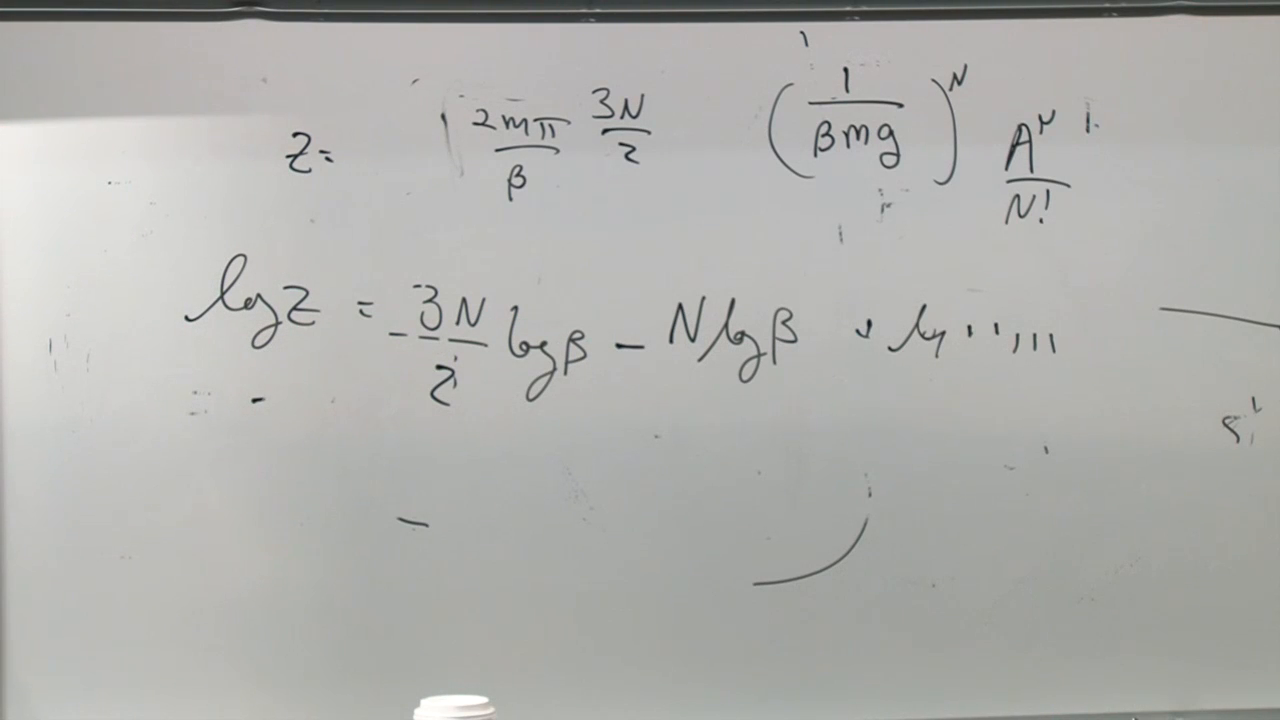
\includegraphics[width=0.83\textwidth]{lecture_04_figure_08.png}
\caption{无限大气配分函数把 \(-N\log\beta\) 加到 \(\log Z\) 上，这就是平均势能的来源。}
\lectureframe{01:36:38}
\end{figure}

\begin{classroomqa}
\audiencequestion{非常强的引力场是否需要另一个拉格朗日乘子？}
\lecturerresponse{并不仅仅因为场强就需要。引力改变哈密顿量，从而改变能级或相空间权重。同一个能量乘子 \(\beta\) 仍然保留。中子星会带来额外的物理复杂性，但第一步修改仍然是把引力势能放入 \(H\)。
\lecturetimestamp{01:27:58--01:29:24}}
\end{classroomqa}

\section{结尾的三个问题}

\begin{classroomqa}
\audiencequestion{哪一个方程是玻尔兹曼分布，它关于平衡断言了什么？}
\lecturerresponse{该分布为
\[
 p_i=\frac{e^{-\beta E_i}}{Z}.
\]
它是在归一化和固定平均能量的约束下具有最大熵的分布。平均能量必须由同一组概率计算，而归一化仍然必须被强制满足，尽管它在最终公式中看起来几乎是自动成立的。
\lecturetimestamp{01:38:14--01:38:45}}
\end{classroomqa}

这套程序可能显得机械：写出配分函数，取对数，然后求导。然而由此得到的方程仍然不断令人惊讶。熟悉会让人知道哪种简单操作应当接在哪种操作之后，但这并不会使这门学科变得不那么奇妙。

\begin{classroomqa}
\audiencequestion{这些熵的思想能应用于坍缩的恒星或黑洞吗？当物质占据更小的区域时，熵怎么能增加？}
\lecturerresponse{恒星之所以困难，主要是因为其物质细节很复杂。黑洞有一个更干净的基准：在给定的宏观约束下，它的贝肯斯坦--霍金熵是极限引力熵。坍缩可以使熵增加，直到达到那个黑洞值；要进一步增加它，就需要改变可用的能量或尺度。
\lecturetimestamp{01:39:29--01:40:36}}
\end{classroomqa}

\begin{classroomqa}
\audiencequestion{配分函数也能计算能量的涨落吗？}
\lecturerresponse{能。一阶导数给出平均能量，二阶导数给出其方差：
\begin{align*}
 \frac{\partial^2\log Z}{\partial\beta^2}
 &=\langle E^2\rangle-\langle E\rangle^2\\
 &=\operatorname{Var}(E).
\end{align*}
以能量单位表示，它与热容的关系为 \(\operatorname{Var}(E)=T^2C_V\)。以实验室单位表示，
\(\operatorname{Var}(E)=k_BT_{\mathrm K}^2C_V\)。这个涨落关系就是下一次计算。
\lecturetimestamp{01:40:37--01:41:53}}
\end{classroomqa}

涨落把统计力学与纯粹连续的热力学描述区分开来。对它们的系统研究尤其与吉布斯和爱因斯坦相关，它揭示了光滑宏观定律背后的有限微观组分。下一讲就从这里开始。